%If possible, give a foreshadowing of possible result outcomes; will they have policy implications?
I use fixed effects regression and synthetic control model to report whether enrollment in the program can improve black students' test scores on different school levels. 

I first run a state-fixed effect regression of black students' math percentage of proficiency against enrollment in the program and a list of control variables. The regression result is summarized in the table below. 

Having a positive coefficient on the variable "enrolled" indicates that the program improved black student's test scores, while a negative coefficient on enrolled means that enrollment in the program decreases black students' math percentage of proficiency.

The regression result in the two tables below is unexpected. Literature and past empirical studies seem to suggest that the implementation of the program will be positive and statistically significantly correlated with an increase in math percentage of proficiency, regardless of school levels. However, my regression result tells a different story. 

\begin{table}[H]\centering
\def\sym#1{\ifmmode^{#1}\else\(^{#1}\)\fi}
\caption{Regression table: black students without control\label{tab1}}
\begin{tabular}{l*{3}{c}}
\hline\hline
  Dependent Variable: &\multicolumn{1}{c}{(1)}&\multicolumn{1}{c}{(2)}&\multicolumn{1}{c}{(3)}\\
black Math Percentage of Proficiency            &\multicolumn{1}{c}{elementary level}&\multicolumn{1}{c}{middle school level}&\multicolumn{1}{c}{high school level}\\
\hline
enrolled    &      -38.25\sym{***}         &       7.286         &      -15\sym{***} \\
            &     (10.464)         &     (6.191)         &     (0.000)         \\
[1em]
constant      &       27.5\sym{***}&       8&       25\\
            &     (1.491)         &     (4.995)         &     (0.000)         \\
\hline
Fixed Effects   &    Y     &Y&Y \\
\hline
\(N\)       &         140         &          53         &          30         \\
adjusted \(R^{2}\)&       0.3490         &       0.0664         &       0.4019         \\
\hline\hline
\multicolumn{4}{l}{\footnotesize Robust standard errors in parentheses}\\
\multicolumn{4}{l}{\footnotesize \sym{*} \(p<0.05\), \sym{**} \(p<0.01\), \sym{***} \(p<0.001\)}\\
\end{tabular}
\end{table}

When not including control variables\footnote{I include regressions without controls because I worry that some of the controls are affected by the intervention themselves.}, on both elementary and high school levels, the coefficient on elementary level is statistically significant but negative, which suggests that the program actually has negative effect on students' academic performance on the elementary level. What's more, coefficient on "enrolled" in the middle school level is statistically insignificant.

After including control variables, while coefficients on "enrolled" are either close to zero or positive, none of the three coefficients is statistically significant. In other words, data can't detect that enrollment in the program has an effect on black student's math performance being significantly different from zero in all three school levels.

\begin{table}[H]\centering
\def\sym#1{\ifmmode^{#1}\else\(^{#1}\)\fi}
\caption{Regression table: black students with control\label{tab1}}
\begin{tabular}{l*{3}{c}}
\hline\hline
  Dependent Variable: &\multicolumn{1}{c}{(1)}&\multicolumn{1}{c}{(2)}&\multicolumn{1}{c}{(3)}\\
black Math Percentage of Proficiency            &\multicolumn{1}{c}{elementary level}&\multicolumn{1}{c}{middle school level}&\multicolumn{1}{c}{high school level}\\
\hline
enrolled    &      -0.0616         &       5.597         &      33.85 \\
            &     (3.800)         &     (6.164)         &     (38.955)         \\
[1em]
Out of School Suspension rate&      13.28         &      -28.73\sym{**} &      -6.977         \\
            &     (21.665)         &     (5.474)         &     (11.741)         \\
[1em]
Math Percentage of Proficiency: ECD&       0.712\sym{***}&       -0.0370         &       0.119 \\
(Economically Disadvantaged students) &    (0.087)         &     (0.172)         &     (0.123)         \\
[1em]
Math Percentage of Proficiency: LEP&     -0.178         &      -0.0856         &       0.546\sym{***}    \\
(Limited English Proficient students)   &    (0.091)         &     (0.207)         &     (0.239)         \\
[1em]
Dropout Rate&              &       &      -38.72      \\
            &             &             &     (56.899)         \\
[1em]
constant      &       8.614&       16.59\sym{***}&       8.647\\
            &     (6.810)         &     (5.234)         &     (16.387)         \\
\hline
Fixed Effects   &    Y     &Y&Y \\
\hline
\(N\)       &         140         &          53         &          30         \\
adjusted \(R^{2}\)&       0.574         &       0.241         &       0.648         \\
\hline\hline
\multicolumn{4}{l}{\footnotesize Robust standard errors in parentheses}\\
\multicolumn{4}{l}{\footnotesize \sym{*} \(p<0.05\), \sym{**} \(p<0.01\), \sym{***} \(p<0.001\)}\\
\end{tabular}
\end{table}




In order to track how the achievement gap changes along with launch of the program, I run another state-fixed effect regression on all school levels of the white-black gap as well. Here, I derive the white-black gap by subtracting black math percentage of proficiency from white math percentage of proficiency, so in most cases, the value should be positive. 

Now, instead of regressing black student's math percentage of proficiency on enrollment of the program and control variables, I regress the white-black gap on the enrollment of the program and a list of control variables that also describe the gap. 

In the regression below, a positive coefficient on the variable "enrolled" indicates that the program works well on closing the achievement gap, while a negative coefficient on enrolled means that enrollment in the program cause the white-black gap to actually be greater.

Tables 5 and 6 still show similar results as the first set of regressions. Before including control variables, on high school level enrollment in the program expands the achievement gap, while on elementary and middle school level there isn't a statistically significant effect.
\begin{table}[H]\centering
\def\sym#1{\ifmmode^{#1}\else\(^{#1}\)\fi}
\caption{Regression table: white-black gap without control\label{tab1}}
\begin{tabular}{l*{3}{c}}
\hline\hline
  Dependent Variable: &\multicolumn{1}{c}{(1)}&\multicolumn{1}{c}{(2)}&\multicolumn{1}{c}{(3)}\\
black Math Percentage of Proficiency            &\multicolumn{1}{c}{elementary level}&\multicolumn{1}{c}{middle school level}&\multicolumn{1}{c}{high school level}\\
\hline
enrolled    &      18        &       -1.929         &      27.5\sym{***} \\
            &     (13.120)         &     (14.187)         &     (0.000)         \\
[1em]
constant      &       -27.5\sym{***}&       29.5\sym{***}&       -5\\
            &     (2.470)         &     (9.373)         &     (0.000)         \\
\hline
Fixed Effects   &    Y     &Y&Y \\
\hline
\(N\)       &         140         &          53         &          30         \\
adjusted \(R^{2}\)&       0.5549         &       0.7306         &       0.8493         \\
\hline\hline
\multicolumn{4}{l}{\footnotesize Robust standard errors in parentheses}\\
\multicolumn{4}{l}{\footnotesize \sym{*} \(p<0.05\), \sym{**} \(p<0.01\), \sym{***} \(p<0.001\)}\\
\end{tabular}
\end{table}

After including control variables, there is no evidence that MDP helps closer the black-white achievement gap on any of the three school levels, as all coefficients on the variable "enrolled" are statistically insignificant. If this is the case, does it suggest that the Manhood Development Program, or the Cultural Relevant Pedagogy, just as past initiatives, doesn't work well in improving black students' academic performance (in this case, math test scores) either?

\begin{table}[H]\centering
\def\sym#1{\ifmmode^{#1}\else\(^{#1}\)\fi}
\caption{Regression table: white-black gap with control\label{tab1}}
\begin{tabular}{l*{3}{c}}
\hline\hline
  Dependent Variable:   &\multicolumn{1}{c}{(1)}&\multicolumn{1}{c}{(2)}&\multicolumn{1}{c}{(3)}\\
  Math Percentage of Proficiency gap           &\multicolumn{1}{c}{elementary gap}&\multicolumn{1}{c}{middle school gap}&\multicolumn{1}{c}{high school gap}\\
\hline
enrolled    &      -6.321         &       -4.913         &       16.23\\
            &     (11.406)         &     (8.021)         &     (8.560)         \\
[1em]
Out of School Suspension rate gap&       -62.27         &       -45.01         &       14.84         \\
            &     (66.880)         &     (30.773)         &     (20.043)         \\
[1em]
Math Percentage of Proficiency: White&       1.258\sym{***}         &       0.872\sym{***}         &        \\
            &     (0.165)         &     (0.225)         &            \\
[1em]
Math Percentage of Proficiency: ECD&       -0.787\sym{***}         &       -0.191         &       0.693  \\
(Economically Disadvantaged students) &     (0.236)         &     (0.468)         &     (0.610)         \\
[1em]
Math Percentage of Proficiency: LEP&      0.297       &       0.296  &      0.611         \\
(Limited English Proficient students)  &     (0.227)         &     (0.522)         &     (0.736)         \\
[1em]
Dropout Rate gap&              &       &      225.1      \\
            &             &             &     (138.602)         \\
[1em]
constant    &       -13.15         &       -10.01         &      -15.55\\
            &     (14.541)         &     (10.032)         &     (7.949)         \\
\hline
Fixed Effects   &    Y     &Y&Y \\
\hline
\(N\)       &          57         &          26         &          14         \\
adjusted \(R^{2}\)&      0.783         &       0.917         &       0.966         \\
\hline\hline
\multicolumn{4}{l}{\footnotesize Standard errors in parentheses}\\
\multicolumn{4}{l}{\footnotesize \sym{*} \(p<0.05\), \sym{**} \(p<0.01\), \sym{***} \(p<0.001\)}\\
\end{tabular}
\end{table}



In order to try to establish a causal relationship between the enrollment in the program and black student's math test scores, I run a synthetic control model on different school levels. 

On the elementary school level, I chose Piedmont Elementary School as the treated unit as this was the first elementary school that MDP was made available to in school year 2013-14. 

The pre-treatment periods are therefore 2011 and 2013, and the post-treatment periods are 2015 and 2017. The donor pool is made up of all other elementary schools in the district that have available data from all school years 2011, 2013, 2015, and 2017. 

Predictors included to construct the synthetic Piedmont Elementary include black Out of School Suspension rate, math Percentage of Proficiency for ECD students and math Percentage of Proficiency for black students in year 2011 and 2013. 

The predictor table for Piedmont Elementary against the synthetic Piedmont Elementary in the pre-treatment period is summarized below.

\begin{table}[H] \centering 
  \caption{} 
  \label{} 
\begin{tabular}{@{\extracolsep{5pt}} cccc} 
\\[-1.8ex]\hline 
\hline \\[-1.8ex] 
 & Treated & Synthetic & Sample Mean \\ 
\hline \\[-1.8ex] 
black Out of School Suspension rate & $0.004$ & $0.004$ & $0.062$ \\ 
Math Percentage of Proficiency: ECD & $77.250$ & $65.276$ & $50.636$ \\ 
\hline \\[-1.8ex] 
\end{tabular} 
\end{table} 

As we can see, the synthetic Piedmont Elementary is very similar to the actual Piedmont Elementary in the pre-treatment period. Table 6 summarizes schools that construct the donor pool and the weight distribution inside the donor pool.

The above table shows that Glenview Elementary and Peralta Elementary make up of most of the weight in the donor pool. 

\begin{table}[H] 
  \centering 
  \caption{} 
  \label{} 
\begin{longtable}{@{\extracolsep{5pt}} cccc}
\\[-1.8ex]\hline 
\hline \\[-1.8ex] 
School Name& School ID & Weight      \\ 
\hline \\[-1.8ex] 
Allendale Elementary & 62805004238 &  0.002 \\
Chabot Elementary & 62805004239 & 0.003  \\
Bella Vista Elementary & 62805004241 &    0.002\\
Brookfield Elementary & 62805004243 &  0.003  \\  
Burckhalter Elementary & 62805004245 &    0.001 \\
Howard Elementary & 62805004249 &    0.002  \\
Cleveland Elementary & 62805004251 &    0.003\\
Emerson Elementary & 62805004260 &   0.002  \\
Franklin Elementary & 62805004261 &    0.018   \\
Fruitvale Elementary & 62805004264 &    0.003 \\
Glenview Elementary & 62805004266 &    0.602 \\
Grass Valley Elementary & 62805004269 &   0.002\\
Kaiser Elementary & 62805004273 &    0.003  \\
Hoover Elementary & 62805004276 &    0.002 \\
Horace Mann Elementary & 62805004277 &    0.004  \\
Joaquin Miller Elementary & 62805004280&   0.003 \\
Laurel Elementary & 62805004287 &   0.002 \\
Lincoln Elementary & 62805004289 &    0.002 \\
Manzanita Community & 62805004294 &   0.001  \\
Markham Elementary & 62805004296 &   0.003\\
Martin Luther King Jr. Elementary & 62805004297 &   0.003\\
Parker Elementary & 62805004306 &   0.003 \\
Peralta Elementary & 62805004307 &  0.312\\
Redwood Heights Elementary & 62805004310 &   0.001 \\
Sequoia Elementary & 62805004314 &   0.002  \\
Madison Park Academy tk-5 & 62805004316 &   0.001  \\
Reach Academy & 62805011556 &    0.001\\
Sankofa Academy & 62805011558 &    0.002  \\
Rise community & 62805011559 &    0.001 \\
Fred T. Korematsu Discovery Academy & 62805011977 &  0.004\\
Futures Elementary & 62805012057 &    0.001  \\
Community United Elementary & 62805012058 &    0.003 \\
East Oakland Pride Elementary & 62805012059 &   0.001  \\
\hline \\[-1.8ex] 
\end{longtable} 
\end{table}

Now, we can take a look at how the black math percentage of proficiency would behave if it had not received the treatment. I first report a table of the period by period comparison between the treated unit and synthetic unit.

\begin{table}[H] \centering 
  \caption{} 
  \label{} 
\begin{tabular}{@{\extracolsep{5pt}} cccc} 
\\[-1.8ex]\hline 
\hline \\[-1.8ex] 
Year& Treated Unit & Synthetic Unit      \\ 
\hline \\[-1.8ex] 
2011&  74.50  &   72.42\\
2013& 54.50 &  56.58 \\
2015  &15.00   & 25.10 \\
2017&  24.50 &    27.95 \\
\hline \\[-1.8ex] 
\end{tabular} 
\end{table}

The following graph shows the path of math percentage of proficiency change for black students over the years.

\begin{figure}[H]
  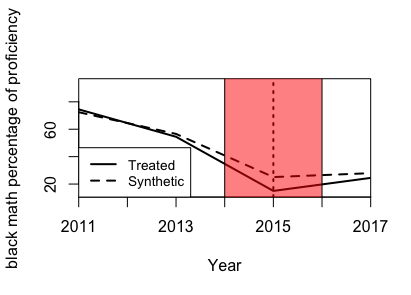
\includegraphics[width=\linewidth]{elementary1.png}
  \caption{Elementary School Level black student math performance}
  \label{fig:boat1}
\end{figure}

In Figure 4, the solid line stands for the treat unit, in this case Piedmont Elementary; the dotted line stands for the synthetic control unit, a synthetic Piedmont Elementary as if it hadn't received the treatment\footnote{The shaded areas means it's uncertain what happened between 2014 and 2016 since I don't have data for 2014 and 2016.Same with the graph for middle school level.}. The figure shows that after 2015, the slope of the treated unit is steeper than the synthetic control unit, which means the program increase black math percentage of proficiency faster than the synthetic unit, a very similar school that didn't receive the treatment. However, I have to admit that there are potential threats to establishing the causal relationship, which I will elaborate in the limitation section.

Next, I move on to the middle school level to investigate whether the synthetic control method can provide a clearer view of the program's impact on black students' math percentage of proficiency. On the middle school level, the treatment unit I chose is the Montera Middle School, the first middle school to launch MDP in school year 2013-2014. By 2015, the program was available to black boys who were in the 8th grade. Therefore, the pre-treatment periods are 2011 and 2013, and the post-treatment periods are 2015 and 2017. Like the elementary school level, the donor pool is made up of middle schools in the district with available data from all school years. 

Predictors included to construct the synthetic Piedmont Elementary include black Out of School Suspension rate, math Percentage of Proficiency for ECD students, Percentage of Proficiency for LEP students, and math Percentage of Proficiency for black students in year 2011 and 2013. The predictor table for Montera Middle against the synthetic "Montera Middle" in the pre-treatment period is summarized below. 

\begin{table}[H] \centering 
  \caption{} 
  \label{} 
\begin{tabular}{@{\extracolsep{5pt}} cccc} 
\\[-1.8ex]\hline 
\hline \\[-1.8ex] 
 & Treated & Synthetic & Sample Mean \\ 
\hline \\[-1.8ex] 
black Out of School Suspension rate & $0.139$ & $0.200$ & $0.292$ \\ 
Math Percentage of Proficiency: ECD& $27$ & $27$ & $19.182$ \\ 
Math Percentage of Proficiency: LEP & $25$ & $13.380$ & $13$ \\ 
\hline \\[-1.8ex] 
\end{tabular} 
\end{table}


Table 12 below summarizes schools composing the donor pool and the weight distribution of schools inside the donor pool. Clearly, Madison Park Academy and Edna Brewer Middle make up of most of the weight in the donor pool, while the weight of other schools in are almost trivial when making up the synthetic Montera Middle. 

\begin{doublespace}
\begin{table}[H] \centering 
  \caption{} 
  \label{} 
\begin{tabular}{@{\extracolsep{5pt}} cccc} 
\\[-1.8ex]\hline 
\hline \\[-1.8ex] 
School Name& School ID & Weight      \\ 
\hline \\[-1.8ex] 
Bret Harte Middle&  62805004242  &   0.039\\
Claremont Middle & 62805004250 &  0.033 \\
Frick Middle  &62805004263   & 0.034 \\
Madison Park Academy&  62805004278 &    0.308 \\
Edna Brewer Middle & 62805004299   &   0.415   \\
Roosevelt Middle  &62805004312   &  0.038   \\
Westlake Middle&  62805004323   & 0.031     \\
Roots International Academy&  62805011907    & 0.025\\
United For Success Academy & 62805011909     &0.025 \\
Elmhurst Community Prep  &62805011961&     0.028  \\
Alliance academy&  62805012027&    0.025   \\
\hline \\[-1.8ex] 
\end{tabular} 
\end{table}
\end{doublespace}

After establishing the synthetic "Montera Middle", I can compare the trend of how the black math percentage of proficiency behaves had it received or not received the treatment. Again, I first report a table of the period by period comparison between the treated unit and synthetic unit.

\begin{doublespace}
\begin{table}[H] \centering 
  \caption{} 
  \label{} 
\begin{tabular}{@{\extracolsep{5pt}} cccc} 
\\[-1.8ex]\hline 
\hline \\[-1.8ex] 
Year& Treated Unit & Synthetic Unit      \\ 
\hline \\[-1.8ex] 
2011&  0.00  &   0.00\\
2013& 17.00 &  17.00 \\
2015  &12.00   & 14.65 \\
2017&  12.00 &    12.33 \\
\hline \\[-1.8ex] 
\end{tabular} 
\end{table}
\end{doublespace}



The solid line in Figure 5 stands for the treat unit, in this case Montera Middle, while the dotted line stands for the synthetic control unit, a synthetic Montera Middle as if it hadn't received the treatment. In Figure 4, we can see both the treated and synthetic control unit have a downward sloping trend after year 2015. This means black students' math percentage of proficiency has a general decreasing trend in those years. 

However, the slope of the treated unit is flatter than the synthetic control unit, which means for the school that has received the treatment suffers from less decline in black students' math percentage of proficiency than the synthetic unit, a very similar hypothetical school that hasn't received the treatment.

\begin{figure}[H]
  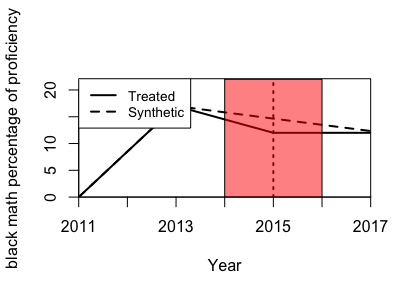
\includegraphics[width=\linewidth]{middle1.png}
  \caption{Middle School Level black student math performance}
  \label{fig:boat1}
\end{figure}

Through the synthetic control method, I find that on both the elementary school and middle school level, MDP has positive impact on black students' math test scores. Finally, I reciprocate the procedure at the high school level to see if there's a similar pattern.

On the high school level, the treatment unit I chose is McClymonds High School, one of the first four high schools to launch MDP in the very beginning. The program was launched first in school year 2011-12 towards the 9th grade cohort. By 2015, the then 9th grade cohort reached the grade to take the state standardized test. Therefore, the pre-treatment periods are 2011 and 2013, and the post-treatment periods are 2015 and 2017. The donor pool is made up of high schools in the district that didn't received the treatment with available data from all school years. Since there are less high schools in general in the district compared with elementary and middle schools, and there are a lot more high schools in the district that have received the treatment (i.e., implemented MDP), the donor pool doesn't have a lot of choices like the elementary and middle school level. The predictor table for McClymonds High against the synthetic "McClymonds High" in the pre-treatment period is summarized below. 

\begin{table}[H] \centering 
  \caption{} 
  \label{} 
\begin{tabular}{@{\extracolsep{5pt}} cccc} 
\\[-1.8ex]\hline 
\hline \\[-1.8ex] 
 & Treated & Synthetic & Sample Mean \\ 
\hline \\[-1.8ex] 
black Out of School Suspension rate & $0.236$ & $0.206$ & $0.172$ \\ 
Math Percentage of Proficiency: ECD & $11$ & $39.750$ & $40.833$ \\ 
black dropout rate & $0.076$ & $0.024$ & $0.015$ \\ 
\hline \\[-1.8ex] 
\end{tabular} 
\end{table} 

Unfortunately, the synthetic "McClymonds High" isn't very similar to the actual McClymonds High during the pre-treatment period since there are only three high schools in the donor pool (as shown in Table 14), and all of the weight in the donor pool is put on Metwest High\footnote{Next step of extending this paper is to include more schools outside of OUSD and I'm confident that in that case synthetic control on the high school level will have a much better result.}.

\begin{table}[H] \centering 
  \caption{} 
  \label{} 
\begin{tabular}{@{\extracolsep{5pt}} cccc} 
\\[-1.8ex]\hline 
\hline \\[-1.8ex] 
School Name& School ID & Weight       \\ 
\hline \\[-1.8ex] 
Life Academy & 62805008676&0\\
Metwest High  &62805011350&1\\
Coliseum College Prep Academy  &62805011920&0\\
\hline \\[-1.8ex] 
\end{tabular} 
\end{table}

I won't report the figure here but when plotting the path overtime, I see that after 2015 both the treated and synthetic control unit have a horizontal line, implying that whether a school receive the treatment or not does not have any impact on black students' math percentage of proficiency. However, I won't read too much into this because the result generated by donor pool is clearly biased.

To sum up, while Fixed Effects regressions suggest no statistically significant evidence on the causal relationship between the launch of the program and black student's math percentage of proficiency, the synthetic control model shows a positive effect of the Manhood Development Program on black student's test scores on the elementary and middle school level. However, there are limitations to both models and I will briefly discuss them in the next section.